\documentclass{beamer}
\usepackage{listings}
\lstset{
%language=C,
frame=single, 
breaklines=true,
columns=fullflexible
}
\usepackage{subcaption}
\usepackage{setspace}
\usepackage{url}
\usepackage{tikz}
\usepackage{tkz-euclide} % loads  TikZ and tkz-base
%\usetkzobj{all}
\usepackage[utf8]{inputenc}
\usepackage{longtable}
\usetikzlibrary{calc,math}
\usepackage{float}
\newcommand\norm[1]{\left\lVert#1\right\rVert}
\renewcommand{\vec}[1]{\mathbf{#1}}
\usepackage[export]{adjustbox}
\usepackage[utf8]{inputenc}
\usepackage{amsmath}
\usetheme{Boadilla}
\newcommand\mytextbullet{\leavevmode%
\usebeamertemplate{itemize item}\hspace{.5em}}

\bibliographystyle{IEEEtran}

\usepackage{color}

\title{Navigation and Communication for UGV/UAV}
\author{Sachinkumar Omprakash Dubey}
\institute{Indian Institute of Technology, Hyderabad.}
\date{\today}
\begin{document}


\begin{frame}
\titlepage
\end{frame}
\section{Content}
\begin{frame}
\frametitle{Content}
\begin{columns}
\column{1\textwidth}
  \begin{itemize}
  \item Introduction
  \item Motor control basic
  \item Serial communication protocols
  \item ESP32 based applications
  \item Vaman based applications
  \item SATCOM for UAV communication
  \item UGV control using NB-IoT setup
  \end{itemize}
\end{columns}

\end{frame}


\section{Introduction}
\begin{frame}
\frametitle{Introduction}
\begin{columns}
\column{1\textwidth}
  \begin{itemize}
  \item In [1-3], the authors have shown various forces on stationary balls with/without spin in wind tunnels of different types. So, \textbf{drag} and \textbf{side} forces are determined.

  \end{itemize}
\end{columns}

\end{frame}


\section{Motor control basic}
\begin{frame}
\frametitle{Motor control basic}


  \begin{itemize}
  \item The trajectory equation is derived from [5], where the author sets an equation for both compact debris and sheet debris.
  
  \end{itemize}


%\begin{columns}
%\column{.5\textwidth}
%  \begin{itemize}
%  \item First item.
%  \item Second item.
%  \end{itemize}
%\end{columns}

\end{frame}

\section{Serial communication protocols}
\begin{frame}
\frametitle{Serial communication protocols}
The basic trajectory equation for cricket balls:\\

\end{frame}

\section{ESP32 Based Applications}
\begin{frame}
\frametitle{ESP32 Based Applications}

\end{frame}

\section{Vaman Based Applications}
\begin{frame}
\frametitle{Vaman Based Applications}
\end{frame}

\section{SATCOM for UAV Communication}
\begin{frame}{SATCOM for UAV Communication}
    \begin{itemize}
    \item 
    When the cricket ball travel through the air towards the batsman, the air flow around the ball can be \textbf{laminar} or \textbf{turbulent}.
  \end{itemize}
\end{frame} 

\section{Conclusion and Future Directions}
\begin{frame}{Conclusion and Future Directions}
    
  
\end{frame} 





%\begin{figure}[h!]
%  \centering
%  \begin{subfigure}[b]{0.5\linewidth}
%    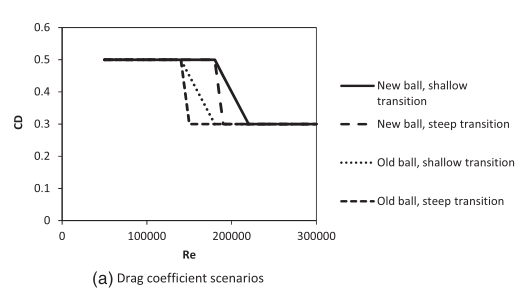
\includegraphics[width=\linewidth]{./figs/my_8.png}
%%    \caption{Coffee.}
%  \end{subfigure}
%  \begin{subfigure}[b]{0.5\linewidth}
%    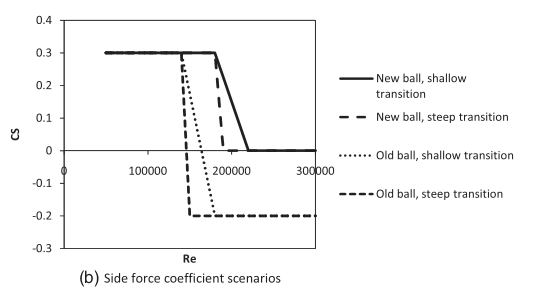
\includegraphics[width=\linewidth]{./figs/my_9.png}
%%    \caption{More coffee.}
%  \end{subfigure}
%  \caption{Force coefficient scenarios for trajectory calculations}
%  \label{fig:side3}
%\end{figure}
%\end{frame}



%\begin{frame}
%
%\begin{columns}
%\column{.5\textwidth}
%  \begin{itemize}
%  \item First item.
%  \item Second item.
%  \item Third item.
%  \end{itemize}
%\setbeamertemplate{itemize items}[square]
%  \begin{itemize}
%  \item First item.
%  \item Second item.
%  \item Third item.
%  \end{itemize}
%\column{.5\textwidth}
%\setbeamertemplate{itemize items}[circle]
%  \begin{itemize}
%  \item First item.
%  \item Second item.
%  \item Third item.
%  \end{itemize}
%\setbeamertemplate{itemize items}[ball]
%  \begin{itemize}
%  \item First item.
%  \item Second item.
%  \item Third item.
%  \end{itemize}
%\end{columns}
%
%\end{frame}

\newpage
\bibliography{ref}

\end{document}

